\documentclass[12pt,xcolor=table,aspectratio=169]{beamer}
\usetheme{Frankfurt}
\usecolortheme{rose}
\usepackage{amsthm}
\usepackage{amsmath}
\usepackage{bbm}
\usepackage{amsfonts}
\usepackage{amssymb}
\usepackage{graphicx}
\usepackage{hyperref}
\usepackage[flushleft]{threeparttable}
\usepackage{tabularx}
\usepackage{booktabs}
\usepackage{siunitx}
\usepackage{tikz}
\usetikzlibrary{decorations.pathreplacing,angles,quotes}
%\usepackage{enumitem}% http://ctan.org/pkg/enumitem

%set up course and number

\newcommand{\ClassName}{TBD}
\newcommand{\ClassNumber}{TBD}
\newcommand{\Topic}{TBD}

% Some optional colors. Change or add as you see fit.
%---------------------------------------------------
 \definecolor{ualbertagreen}{HTML}{007C41}
\definecolor{ualbertagold}{HTML}{FFDB05}

\definecolor{calloutgrey}{HTML}{D9D9D9}


%set fonts
\setbeamerfont{subtitle}{size=\large,shape=\scshape,series=\bfseries}
\setbeamerfont{title}{size=\Large,shape=\scshape,series=\bfseries}
\setbeamerfont{author}{size=\large}
\setbeamerfont{date}{size=\large}
\setbeamerfont{caption}{size=\scriptsize}


% Some optional color adjustments to Beamer. Change as you see fit.
%------------------------------------------------------------------
\setbeamercolor{frametitle}{fg=ualbertagreen,bg=white}
\setbeamercolor{title}{fg=ualbertagreen,bg=white}
\setbeamercolor{author}{fg=ualbertagreen,bg=white}
\setbeamercolor{date}{fg=ualbertagreen,bg=white}
\setbeamercolor{local structure}{fg=ualbertagreen}
\setbeamercolor{section in toc}{fg=ualbertagreen,bg=white}
% \setbeamercolor{subsection in toc}{fg=ualbertagreen,bg=white}
\setbeamercolor{footline}{fg=ualbertagreen!50, bg=white}

% definition boxes
\setbeamercolor{block title}{bg=ualbertagreen,fg=white}
\setbeamercolor{block body}{parent=normal text,use=block title,bg=calloutgrey}
%\setbeamercolor{block body}{parent=normal text,use=block title,bg=block title.bg!30!bg}


\setbeamercolor{upper separation line head}{bg=ualbertagreen}
\setbeamercolor{lower separation line head}{bg=ualbertagold}
\setbeamercolor{middle separation line head}{bg=ualbertagold}
\setbeamercolor{frametitle}{fg=ualbertagreen,bg=white}



\setbeamercolor{section in head/foot}{bg=white,fg=ualbertagreen}
\setbeamercolor{author in head/foot}{bg=white,fg=ualbertagreen}
\setbeamercolor{date in head/foot}{bg=white,,fg=ualbertagreen}
\setbeamercolor{title in head/foot}{bg=white,fg=ualbertagreen}

\setbeamercolor{headline}{bg=white,fg=ualbertagreen}




\setbeamercolor*{middle separation line head}{bg=ualbertagreen}
\setbeamercolor*{alerted text}{fg=ualbertagreen}
\setbeamercolor*{example text}{fg=black}
\setbeamercolor*{structure}{fg=black}


\let\Tiny=\tiny



\logo{
   %\ifnum\insertpagenumber>1
   \tikz [remember picture,overlay]
    \node[yshift=.3cm,xshift=1.5cm] at (current page.south west)
        %or: (current page.center)
        {
\includegraphics[width=1in]{../images/UA-ASB-COLOUR.png}};
    %\fi
%
\includegraphics[height=0.8cm]{../images/UA-ASB-COLOUR.png}\vspace{220pt}
}


\setbeamertemplate{title page}{%
  \vbox{}
    \vspace{.5cm}% NEW
  \begingroup
    \centering
    \begin{beamercolorbox}[sep=8pt,center]{title}
      \usebeamerfont{title}\ClassNumber: \ClassName\par%
      \usebeamerfont{title}\inserttitle\par%
     \ifx\insertsubtitle\@empty%
      \else%
        \vskip0.05em%
        {\usebeamerfont{subtitle}\usebeamercolor[fg]{subtitle}\insertsubtitle\par}%
      \fi%
    \end{beamercolorbox}%
    \begin{beamercolorbox}[sep=8pt,center]{author}
      \usebeamerfont{author}\insertauthor
    \end{beamercolorbox}
    \begin{beamercolorbox}[sep=8pt,center]{institute}
      \usebeamerfont{institute}\insertinstitute
    \end{beamercolorbox}

    \vspace{0.5cm}% NEW
    \begin{beamercolorbox}[sep=8pt,center]{date}
      \usebeamerfont{date}\insertdate
    \end{beamercolorbox}\vskip0.05em

      \endgroup
  %\vfill
}


\setbeamertemplate{frametitle}{%
    \insertframetitle\par\vskip-10pt
}



\renewcommand{\ClassName}{Business Economics, Organization and Management}
\renewcommand{\ClassNumber}{BUEC 311}

\setbeamertemplate{headline}{%
\leavevmode%
 \hbox{%
    \begin{beamercolorbox}[wd=\paperwidth,ht=5ex,dp=0ex]{white}%
    \usebeamerfont{headline}\hskip6pt\ClassNumber: \inserttitle\par%
    \insertsectionnavigationhorizontal{\paperwidth}{}{\hskip0pt plus1filll}
    \end{beamercolorbox}%
  }
}

\defbeamertemplate*{footline}{my footline}{%
    \ifnum\insertpagenumber=1
        \Tiny{%
            \hfill%
		\vspace*{1pt}%
            %\insertframenumber/\inserttotalframenumber \hspace*{0.1cm}%
            \newline%
            \color{ualbertagold}{\rule{\paperwidth}{0.4mm}}\newline%
            \color{ualbertagold}{\rule{\paperwidth}{.4mm}}%
        }
  \else%
        \Tiny{%
            \hspace{.66\paperwidth}
            %\vspace{25pt}
            \insertframenumber/\inserttotalframenumber
            \newline%
            \color{ualbertagold}{\rule{\paperwidth}{0.4mm}}\newline%
            \color{ualbertagold}{\rule{\paperwidth}{.4mm}}%
        }%
    \fi%
}


\newenvironment{itemize*}%
  {\begin{itemize}%
    \setlength{\itemsep}{0pt}%
    \setlength{\parskip}{0pt}}%
  {\end{itemize}}


\title{Strategic Behaviour Part 2\\
	Strategies Over Time and Dynamic Games
}

\date{Fall 2020}

\begin{document}

\frame{
	\titlepage
}

\frame{
	\frametitle{Outline}
	\begin{enumerate}
	\item Overview
	\item[]
	\item Repeated Games
	\item[]
	\item Sequential Games
	\item[]
	\item Deterring Entry
	\item[]
	\item Cost and Innovation Strategies
	\item[]
	\item Disadvantages of Moving First
	\item[]
	\item Behavioural Game Theory
	\end{enumerate}
}

\frame{
	\frametitle{Outline}
	\begin{enumerate}
	\item \alert{Overview}
	\item[]
	\item Repeated Games
	\item[]
	\item Sequential Games
	\item[]
	\item Deterring Entry
	\item[]
	\item Cost and Innovation Strategies
	\item[]
	\item Disadvantages of Moving First
	\item[]
	\item Behavioural Game Theory
	\end{enumerate}
}

\frame{
	\frametitle{1. Strategic Interaction Over Time}
	\begin{itemize}
	\item Last topic: Strategic interaction in static setting.
		\begin{itemize}
		\item But in practice, many interactions occur \underline{dynamically} over time.
		\end{itemize}
	\item[]
	\item \underline{Dynamic games}: Games where players play the game over and over, and move either \underline{repeatedly} or \underline{sequentially}.
	\end{itemize}
}

\frame{
	\frametitle{Outline}
	\begin{enumerate}
	\item Overview
	\item[]
	\item \alert{Repeated Games}
	\item[]
	\item Sequential Games
	\item[]
	\item Deterring Entry
	\item[]
	\item Cost and Innovation Strategies
	\item[]
	\item Disadvantages of Moving First
	\item[]
	\item Behavioural Game Theory
	\end{enumerate}
}

\frame{
	\frametitle{2. Repeated Games}
	\begin{itemize}
	\item A repeated game is a game in which a static \textit{constituent} game is repeated a finite and pre-specified number of times, or is repeated indefinitely.
	\item[]
	\item We still need to know:
		\begin{itemize}
		\item Players
		\item Rules
		\item Information
		\item Payoffs
		\end{itemize}
	\item[]
	\item Key difference from a static game: How we think about actions and strategies.
	\end{itemize}
}

\frame{
	\frametitle{2. Repeated Games}
	\begin{itemize}
	\item In a repeated game:
		\begin{itemize}
		\item An \underline{action} is a single move that a player makes at a specified time, such as choosing an output level or a price.
		\item[]
		\item A \underline{strategy} is a battle plan that specifies the \textit{full set} of actions that a player will make throughout the game.
			\begin{itemize}
			\item It may involve actions that are conditional on prior actions of other players, or on new information available at a given time.
			\end{itemize}
		\end{itemize}
	\end{itemize}
}

\frame{
	\frametitle{2. Repeated Games}
	\begin{itemize}
	\item As an example, we will revisit game between American and United.
	\item[]
	\item Recall: The Nash equilibrium in the static game is both firms producing high (64k passengers) and making \$4.1 million.
	\end{itemize}
}

\frame{
	\frametitle{2. Repeated Games}
	\begin{figure}
	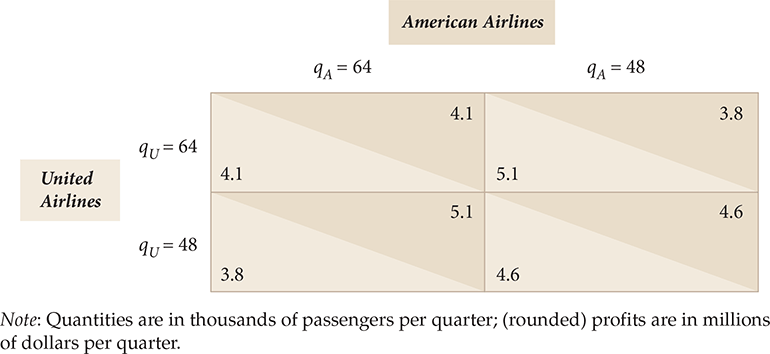
\includegraphics[scale=0.4]{../images/game_theory/oligopoly.png}
	\end{figure}
}

\frame{
	\frametitle{2. Repeated Games}
	\begin{itemize}
	\item Now assume that the same game gets \underline{repeated indefinitely}.
		\begin{itemize}
		\item Now firms must consider both current and future profits.
		\end{itemize}
	\item[]
	\item With repetition, the outcome may be different than in the static game.
		\begin{itemize}
		\item Depends on the strategies used by the firms.
		\end{itemize}
	\end{itemize}
}

\frame{
	\frametitle{2. Repeated Games}
	\begin{itemize}
	\item Suppose, for example, that American adopts the following strategy:
		\begin{itemize}
		\item It cheap-talks United that it will produce the collusive or cooperative quantity of 48k in the first period.
		\item But its subsequent decisions depend on United:
			\begin{itemize}
			\item If United produces 48k in period $t$, American will produce 48k in period $t+1$.
			\item If United produces 64k in period $t$, American will produce 64k in period $t+1$.
			\end{itemize}
		\end{itemize}
	\item[]
	\item What is United's best response to this strategy?
	\end{itemize}
}

\frame{
	\frametitle{2. Repeated Games}
	\begin{figure}
	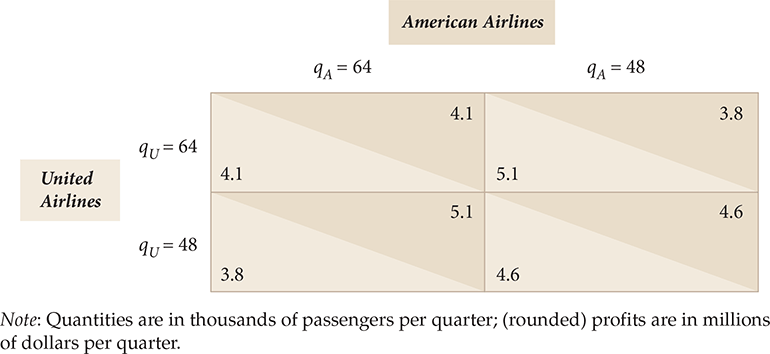
\includegraphics[scale=0.4]{../images/game_theory/oligopoly.png}
	\end{figure}
}

\frame{
	\frametitle{2. Repeated Games}
	\begin{itemize}
	\item American's strategy is an example of a \underline{trigger strategy}.
		\begin{itemize}
		\item Trigger strategy: Rival's defection from a collusive outcome \textit{triggers} punishment.
		\end{itemize}
	\item[]
	\item If United adopts the same trigger strategy, the Nash-equilibrium is the collusive outcome.
		\begin{itemize}
		\item Neither firm has an incentive to deviate.
		\item One period gains from doing so are not sufficient to offset all future losses.
		\end{itemize}
	\item[]
	\item In reality, cooperation may not be sustainable because of regulation, bounded rationality, or if the firm cares little about future profits.
	\end{itemize}
}

\frame{
	\frametitle{2. Repeated Games}
	\begin{itemize}
	\item Trigger strategy is just one possible option for American.
	\item[]
	\item They could instead adopt a \underline{tit-for-tat} strategy.
		\begin{itemize}
		\item Tit-for-tat: Cooperate in first round, then copy rival's action in each subsequent round.
		\end{itemize}
	\item[]
	\item Tit-for-tat may induce cooperation if the payoff from deviating in any period is less than the loss from punishment in the subsequent period.
		\begin{itemize}
		\item It depends on how firms discount the future.
		\end{itemize}
	\item[]
	\item Cooperation is also more likely if the tit-for-tat strategy is modified to extend punishment for more than one period.
		\begin{itemize}
		\item Extension of punishment needs to offset the one-time gains from not cooperating.
		\end{itemize}
	\end{itemize}
}

\frame{
	\frametitle{2. Repeated Games}
	\begin{itemize}
	\item The equilibrium of the repeated game between American and United is an example of a collusive outcome.
	\item[]
	\item In most modern economies, explicit collusion is illegal.
		\begin{itemize}
		\item However, antitrust and competition laws typically do not strictly prohibit choosing the cooperative (or cartel) quantity or price as long as no \underline{explicit} agreement is reached.
		\item Firms may be able to engage in \underline{implicit collusion} or \underline{tacit collusion} using trigger, tit-for-tat, or other similar strategies, as long as firms do not explicitly communicate with each other.
			\begin{itemize}
			\item Tacit collusion lowers society's total surplus just as explicit collusion does.
			\end{itemize}	
		\end{itemize}
	\end{itemize}
}

\frame{
	\frametitle{2. Repeated Games}
	\begin{itemize}
	\item Sustaining the cooperative outcome requires that players believe the game will repeat for ever.
	\item[]
	\item if there is a known end to the game, and players have complete foresight, the cooperation can be impossible to maintain.
	\end{itemize}
}

\frame{
	\frametitle{2. Repeated Games}
	\begin{itemize}
	\item  To see this, suppose that American and United know that they will play the game a finite number of times ($T$).
	\item[]
	\item Suppose both firms use the trigger strategy that sustained collusion when the game was infinitely repeated.
	\item[]
	\item Now, the trigger strategy does not lead to a Nash Equilibrium.
	\item[]
	\item Why not?
	\end{itemize}
}

\frame{
	\frametitle{2. Repeated Games}
	\begin{figure}
	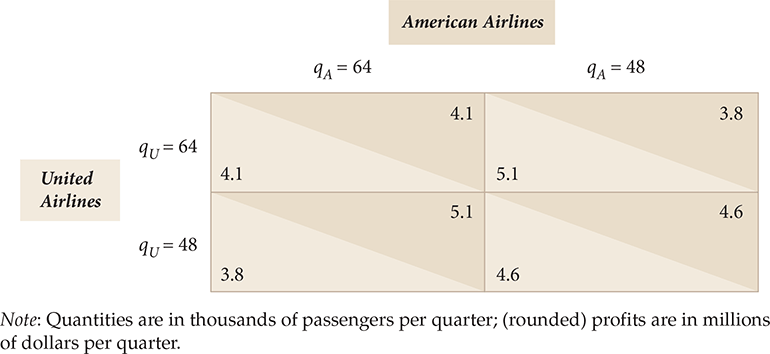
\includegraphics[scale=0.4]{../images/game_theory/oligopoly.png}
	\end{figure}
}

\frame{
	\frametitle{2. Repeated Games}
	\begin{itemize}
	\item When the game is repeated a finite number of times, the only Nash Equilibrium is for both firms to produce a high level of output in all periods.
		\begin{itemize}
		\item There is no cooperation again.
		\end{itemize}
	\end{itemize}
}

\frame{
	\frametitle{Outline}
	\begin{enumerate}
	\item Overview
	\item[]
	\item Repeated Games
	\item[]
	\item \alert{Sequential Games}
	\item[]
	\item Deterring Entry
	\item[]
	\item Cost and Innovation Strategies
	\item[]
	\item Disadvantages of Moving First
	\item[]
	\item Behavioural Game Theory
	\end{enumerate}
}

\frame{
	\frametitle{3. Sequential Games}
	\begin{itemize}
	\item So far, we've maximized strategic interactions where players make simultaneous decisions.
	\item[]
	\item But in many interactions, players alternate moves.
	\item[]
	\item We can model this type of strategic interaction as a \underline{sequential game}.
	\end{itemize}
}

\frame{
	\frametitle{3. Sequential Games}
	\begin{itemize}
	\item As an example, we will again revisit the interaction between American and United, but we will now assume that the firms move sequentially in two stages:
		\begin{itemize}
		\item First, American (the \underline{leader}) chooses its output level.
		\item Second, United (the \underline{follower}) chooses its output level.
		\end{itemize}
	\item[]
	\item This is an example of a \underline{Stackelberg} oligopoly.
		\begin{itemize}
		\item Stackelberg oligopoly involves one leader and one or more followers.
		\end{itemize}
	\end{itemize}
}

\frame{
	\frametitle{3. Sequential Games}
	\begin{figure}
	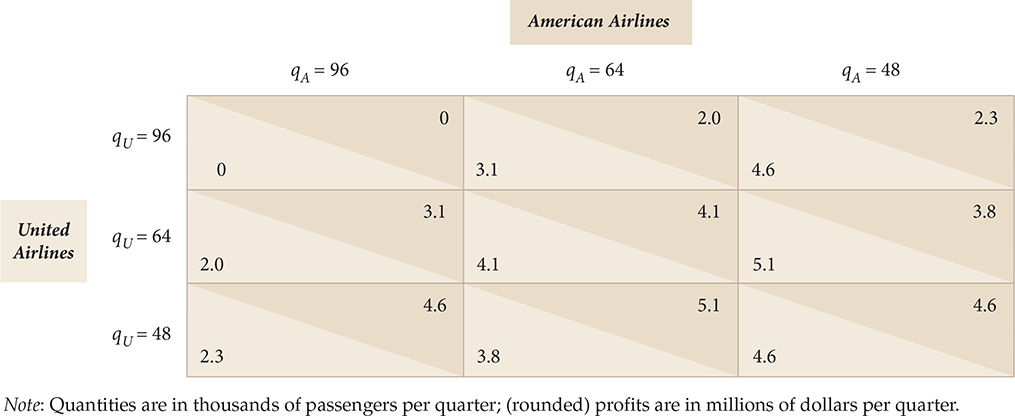
\includegraphics[scale=0.35]{../images/game_theory/stackelberg.png}
	\caption{Payoffs in the Stackelberg game}
	\end{figure}
}

\frame{
	\frametitle{3. Sequential Games}
	\begin{itemize}
	\item Key issue with the payoff matrix:
		\begin{itemize}
		\item It does not show the sequential nature of the game.
		\end{itemize}
	\item[]
	\item We can better illustrate the game using an extensive form diagram.
		\begin{itemize}
		\item Also known as a game tree, or a decision tree.
		\item The extensive form is a branched diagram that shows the players, the sequence of moves, the actions players can take at each move, the information that each player has about previous moves, and the payoff function over all possible strategy combinations.
		\end{itemize}
	\end{itemize}
}

\frame{
	\frametitle{3. Sequential Games}
	\begin{figure}
	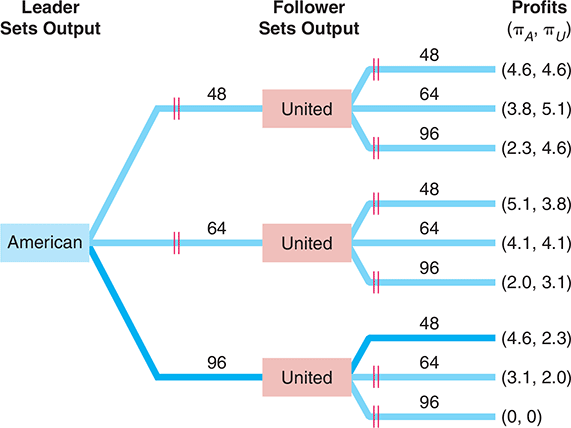
\includegraphics[scale=0.4]{../images/game_theory/stackelberg_tree.png}
	\end{figure}
}

\frame{
	\frametitle{3. Sequential Games}
	\begin{itemize}
	\item The sequential game depicted in the extensive form has four \underline{subgames}.
	\item[]
	\end{itemize}
	\begin{definition}[Subgame]
	A subgame consists of all of the actions (and the corresponding payoffs) that a player can take at a given stage in the game, \textit{given the actions that have already been taken}.
	\end{definition}
}

\frame{
	\frametitle{3. Sequential Games}
	\begin{itemize}
	\item To predict the outcome of the sequential game, we need to know the set of strategies that form a Nash equilibrium in each subgame.
		\begin{itemize}
		\item These strategies yield the \underline{subgame-perfect Nash Equilibrium}.
		\end{itemize}
	\item[]
	\item We can solve for the subgame-perfect Nash Equilibrium through backward induction.
		\begin{itemize}
		\item First, we determine the best response by the last player to move, then we determine the best response for the player who makes the next-to-last move, and so on, until we reach the first move of the game.
		\end{itemize}
	\end{itemize}
}

\frame{
	\frametitle{3. Sequential Games}
	\begin{figure}
	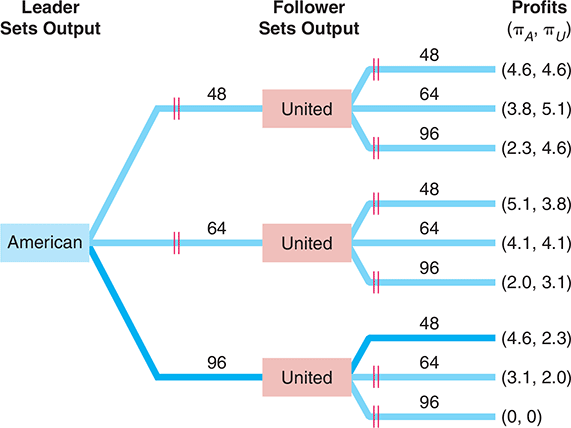
\includegraphics[scale=0.4]{../images/game_theory/stackelberg_tree.png}
	\end{figure}
}

\frame{
	\frametitle{3. Sequential Games}
	\begin{itemize}
	\item In the game between American and United, American first determines what United (the follower), will do in the second stage of the game in each of the three subgames.
		\begin{itemize}
		\item This is the $q_U$ with the highest profit at each node.
		\end{itemize}
	\item[]
	\item American then determines the best action in the first stage given the choices that United will make \textit{conditional on its actions} in the second stage.
		\begin{itemize}
		\item This amounts to choosing the $q_A$ with the highest profit.
		\end{itemize}
	\item[]
	\item Thus, American chooses $q_A = 96$ in the first stage, and United chooses $q_U =48$ in the second stage.
		\begin{itemize}
		\item This is a subgame perfect Nash equilibrium; neither firm wants to change its strategy given what the other player is doing.
		\end{itemize}
	\end{itemize}
}

\frame{
	\frametitle{3. Sequential Games}
	\begin{itemize}
	\item It is worth noting that if this game was played simultaneously, the Nash equilibrium would be $q_{A}=q_{U}=64$.
	\item[]
	\item Simultaneous and sequential games have different solutions because of credible threats and first mover advantage.
		\begin{itemize}
		\item For a firm's strategy to be a \underline{credible threat}, rivals must believe that the firm's strategy is rational (that is, it works in the firm's best interest).
		\item In the simultaneous move game between United and American, United will not believe a threat by American to produce 96. However, in the sequential game, commitment to produce 96 is credible because American makes the first move.
		\end{itemize}
	\end{itemize}
}

\frame{
	\frametitle{Outline}
	\begin{enumerate}
	\item Overview
	\item[]
	\item Repeated Games
	\item[]
	\item Sequential Games
	\item[]
	\item \alert{Deterring Entry}
	\item[]
	\item Cost and Innovation Strategies
	\item[]
	\item Disadvantages of Moving First
	\item[]
	\item Behavioural Game Theory
	\end{enumerate}
}

\frame{
	\frametitle{4. Deterring Entry}
	\begin{itemize}
	\item The Stackleberg game demonstrates the leader can benefit from moving before followers.
	\item[]
	\item In some markets, by moving first, a firm can act strategically to deter a (potential) rival from entering the market.
	\item[]
	\item Two possible approaches:
		\begin{enumerate}
		\item Exclusion contracts.
		\item Limit pricing.
		\end{enumerate}
	\end{itemize}
}

\frame{
	\frametitle{4. Deterring Entry}
	\begin{itemize}
	\item As an example of an exclusion contract, suppose a mall has a single shoe store, the \underline{incumbent} firm.
		\begin{itemize}
		\item The incumbent has an option to pay the mall's owner to add a clause to its rental agreement that guarantees \underline{exclusivity}.
			\begin{itemize}
			\item In the incumbent pays $b$, the landlord agrees to rent remaining space to non-shoe firms.
			\end{itemize}
		\item[]
		\item If the rental agreement does not guarantee exclusivity, a \underline{potential rival} can decide whether to enter.
			\begin{itemize}
			\item If the rival enters, it incurs a fixed fee of $F$ to build its store in the mall.
			\end{itemize}
		\item[]
		\item This interaction can be viewed as a two-stage game.
		\end{itemize}
	\end{itemize}
}

\frame{
	\frametitle{4. Deterring Entry}
	\begin{figure}
	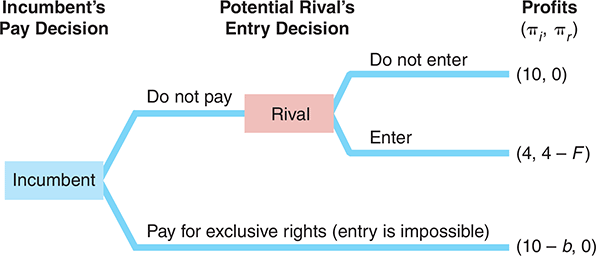
\includegraphics[scale=0.4]{../images/game_theory/entry.png}
	\end{figure}
}

\frame{
	\frametitle{4. Deterring Entry}
	\begin{itemize}
	\item Should the incumbent pay for the exclusive contract?
	\item[]
	\item It depends on the values of $b$ and $F$:
		\begin{enumerate}
		\item \underline{Blockaded entry} $(F>4)$: Potential rival will stay out, ensuring $\pi_{r}=0$. Incumbent avoids paying $b$ and still earn monopoly profit of $\pi_{i}=10$.
		\item \underline{Deterred entry} $(F\leq4,b\leq6)$: Potential rival will enter unless the incumbent pays the exclusivity fee. The incumbent chooses to pay $b$ because $b\leq6$ ensures a profit that is at least as large as the duopoly profit of $4$ ($\pi_{i}=10-b \geq 4$).
		\item \underline{Accommodated entry} $(F\leq4,b>6)$: Potential rival will enter and earn a positive profit of $\pi_{r} = 4-F$. The incumbent does not pay the exclusivity fee because $b$ is so high that it is better to ensure $\pi_i=4$ than earn less ($\pi_{i}=10-b < 4$).
		\end{enumerate}
	\item[]
	\item The incumbent will only pay if it is profit maximizing to do so.
	\end{itemize}	
}

\frame{
	\frametitle{4. Deterring Entry}
	\begin{itemize}
	\item In many industries, it may not be possible to deter entry.
	\item[]
	\item Instead, firms may try to \textit{delay} entry.
		\begin{itemize}
		\item Example: Pharmaceutical companies in the U.S.
			\begin{itemize}
			\item When drug patents expire, the first company to file with FDA has 180-day window to be exclusive producer of generic drug. After 180 days, other generics can enter.
			\item Companies with expired patents used pay-to-delay schemes to prevent entry of generics. Firms pay potential competitors to not enter the market.
			\item The US supreme court ruled this was illegal \textit{if} it violated antitrust.
			\item The FTC has pursued some firms; they reached a \$1.2 billion dollar settlement with Teva Ltd to compensate purchasers of Provigil who paid high prices due to pay-to-delay agreement.
			\end{itemize}
		\end{itemize}
	\end{itemize}
}

\frame{
	\frametitle{4. Deterring Entry}
	\begin{itemize}
	\item Alternative deterrence strategy: Limit Pricing
		\begin{itemize}
		\item A firm is \underline{limit pricing} if it sets its price (or equivalently, its output) os that another firm cannot enter the market profitably.
		\item[]
		\item Credible limit pricing requires the firm to have an advantage over its rivals.
			\begin{itemize}
			\item Ex: A monopolist with a significant cost advantage can threaten to reduce its price if another firm enters to the point where entrant makes a loss.
			\item Ex: A Stackleberg leader can act first and commit to producing a large enough quantity to ensure that any follower would earn no profit.
			\end{itemize}
		\end{itemize}
	\end{itemize}
}

\frame{
	\frametitle{4. Deterring Entry}
	\begin{itemize}
	\item Entry games can be repeated over time or over space.
		\begin{itemize}
		\item A profitable firm will likely face repeated entry threats from potential rivals over time/locations.
		\end{itemize}
	\item[]
	\item Example: A grocery chain with a monopoly in many small towns.
		\begin{itemize}
		\item Chain may face entry in some, or all locations.
		\item Two stage game:
			\begin{enumerate}
			\item Rival decides on entry.
			\item Incumbent decides to accommodate or fight.
			\end{enumerate}
		\item Outcome depends on repetition, level of information.
		\end{itemize}
	\end{itemize}
}


\frame{
	\frametitle{4. Deterring Entry}
	\begin{figure}
	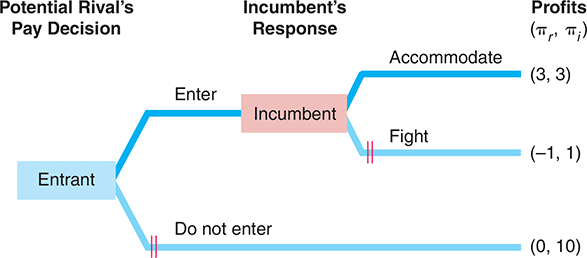
\includegraphics[scale=0.4]{../images/game_theory/grocery.png}
	\end{figure}
}

\frame{
	\frametitle{4. Deterring Entry}
	\begin{itemize}
	\item The incumbent will accommodate if the game is played once, and profits are common knowledge.
	\item[]
	\item The incumbent will still accommodate if the game is repeated and profits are common knowledge.
		\begin{itemize}
		\item If profits are common knowledge, rival knows that fighting each time is not rational.
		\end{itemize}
	\item[]
	\item If profits are not common knowledge and game is repeated, the best strategy may be for incumbent to fight.
		\begin{itemize}
		\item Fighting builds reputation.
		\item Can be part of a subgame perfect Nash equilibrium in which entry is deterred.
		\end{itemize}
	\end{itemize}
}

\frame{
	\frametitle{Outline}
	\begin{enumerate}
	\item Overview
	\item[]
	\item Repeated Games
	\item[]
	\item Sequential Games
	\item[]
	\item Deterring Entry
	\item[]
	\item \alert{Cost and Innovation Strategies}
	\item[]
	\item Disadvantages of Moving First
	\item[]
	\item Behavioural Game Theory
	\end{enumerate}
}

\frame{
	\frametitle{5. Cost and Innovation Strategies}
	\begin{itemize}
	\item Another benefit to moving first: potential to gain a cost advantage over a rival.
	\item[]
	\item Two cases:
		\begin{enumerate}
		\item Lowering own marginal cost.
		\item Increasing rival's marginal cost by more than own.
		\end{enumerate}
	\end{itemize}
}

\frame{
	\frametitle{5. Cost and Innovation Strategies}
	\begin{itemize}
	\item Previously, we discussed \underline{process innovation} as a means to reduce marginal costs.
		\begin{itemize}
		\item Invest if profit from reduced $MC$ exceeds the cost of innovation.
		\end{itemize}
	\item[]
	\item Important secondary motive for process innovation: deterring entry.
		\begin{itemize}
		\item This can provide justification for investment even if the profit from lower $MC$ does not exceed the cost of innovation.
		\end{itemize}
	\end{itemize}
}

\frame{
	\frametitle{5. Cost and Innovation Strategies}
	\begin{itemize}
	\item Example: A monopoly considers investment (installing robots on its assembly line) that would lower marginal costs.
		\begin{itemize}
		\item The threat of entry may induce the monopolist to invest even though it will reduce profits.
		\end{itemize}
	\end{itemize}	
}	

\frame{
	\frametitle{5. Cost and Innovation Strategies}
	\begin{figure}
	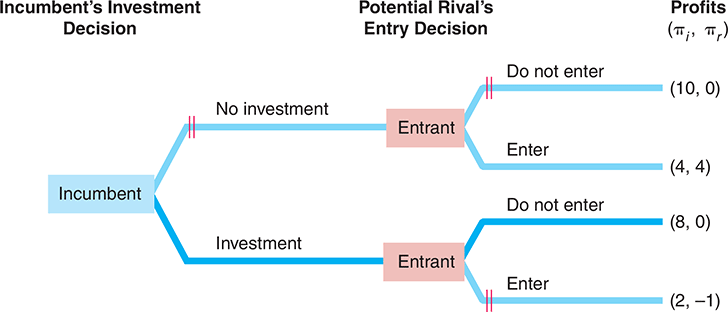
\includegraphics[scale=0.5]{../images/game_theory/robots.png}
	\end{figure}
}

\frame{
	\frametitle{5. Cost and Innovation Strategies}
	\begin{itemize}
	\item Learning by doing can also induce strategic behaviour.
		\begin{itemize}
		\item In the presence of learning by doing, the first firm in the market may want to produce more than the short-run profit maximizing quantity so that its marginal cost is lower than that of a late-entering rival.
		\end{itemize}
	\item[]
	\item Two examples:
		\begin{enumerate}
		\item Aircraft: Price of Lockheed L-1011 was below static $MC$ for most of production run because of steep learning curve.
		\item Computer chips: AMD?s cost of producing computer chips was about 12\% higher than Intel because of less learning by doing.
		\end{enumerate}
	\end{itemize}
}

\frame{
	\frametitle{5. Cost and Innovation Strategies}
	\begin{itemize}
	\item Firms may also benefit from adopting a strategy that raises own cost, but raises rivals? cost by more.
		\begin{itemize}
		\item Such strategies usually favour the first mover, or incumbent.
		\end{itemize}
	\item[]
	\item Strategies for incumbents to raise rival?s costs:
		\begin{enumerate}
		\item \underline{Lobby} the government for more industry regulations that raise costs, as long as the legislation \underline{grandfathers} existing firm's plants.
		\item Increase the \underline{cost of switching} by imposing a switching fee to customers that take their business elsewhere or designing products that don't work with those of rivals.
		\item Use \underline{patents} to prevent rivals from entering the market and increasing competition.
		\end{enumerate}
	\end{itemize}
}

\frame{
	\frametitle{Outline}
	\begin{enumerate}
	\item Overview
	\item[]
	\item Repeated Games
	\item[]
	\item Sequential Games
	\item[]
	\item Deterring Entry
	\item[]
	\item Cost and Innovation Strategies
	\item[]
	\item \alert{Disadvantages of Moving First}
	\item[]
	\item Behavioural Game Theory
	\end{enumerate}
}

\frame{
	\frametitle{6. Disadvantages of Moving First}
	\begin{itemize}
	\item While moving first can create many advantages, it is not always beneficial.
	\item[]
	\item One potential disadvantage: the \underline{holdup problem}.
		\begin{itemize}
		\item The holdup problem arises when two firms want to contract or trade with each other but one firm must move first by making a \underline{specific investment} (can only be used in its transaction with the second firm).
			\begin{itemize}
			\item Problem: The second firm can take advantage of the first.
			\item If the first firm does not anticipate the opportunistic behaviour and invests, it may earn no profit.
			\item If the first firm anticipates the opportunistic behaviour and does not invest, both firms lose.
			\end{itemize}
		\end{itemize}
	\end{itemize}
}

\frame{
	\frametitle{6. Disadvantages of Moving First}
	\begin{figure}
	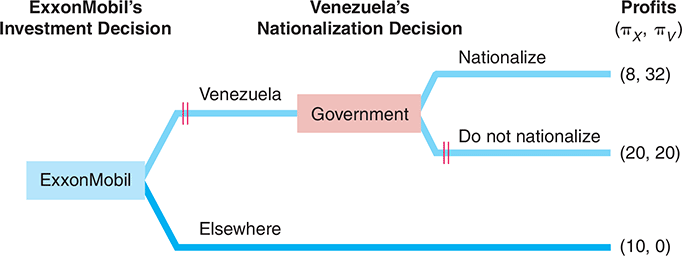
\includegraphics[scale=0.5]{../images/game_theory/venezuela.png}
	\caption{Venezuela - Exxon-Mobile Holdup Problem}
	\end{figure}
}

\frame{
	\frametitle{6. Disadvantages of Moving First}
	\begin{itemize}
	\item There are several possible strategies for avoiding the holdup problem.
		\begin{enumerate}
		\item Contracts
		\item Vertical integration.
		\item Quasi-vertical integration.
		\item Reputation building.
		\item Multiple/open sourcing.
		\end{enumerate}
	\end{itemize}
}

\frame{
	\frametitle{6. Disadvantages of Moving First}
	\begin{itemize}
	\item Another potential disadvantage of moving first: too-early product innovation.
		\begin{itemize}
		\item Advantage of innovating and creating new product: \underline{customer loyalty}. Later entrants find it difficult to take market share away from the leader.
		\item But entering with a new product too early can raise costs, increase the odds of miscalculating demand, and later rivals may build on the leader's research to produce a superior product.
		\end{itemize}
	\item[]
	\item Example: Tagamet.
		\begin{itemize}
		\item Tagamet was the first entrant of a new class of anti-ulcer drugs; it was extremely successful when introduced.
		\item Zantac, the second entrant, rapidly took over the market.
		\item Tagamet moved too early; Zantac had fewer side effects, needed to be taken less frequently, and was promoted more effectively.
		\end{itemize}
	\end{itemize}
}

\frame{
	\frametitle{Outline}
	\begin{enumerate}
	\item Overview
	\item[]
	\item Repeated Games
	\item[]
	\item Sequential Games
	\item[]
	\item Deterring Entry
	\item[]
	\item Cost and Innovation Strategies
	\item[]
	\item Disadvantages of Moving First
	\item[]
	\item \alert{Behavioural Game Theory}
	\end{enumerate}
}

\frame{
	\frametitle{7. Behavioural Game Theory}
	\begin{itemize}
	\item While it is reasonable to assume that people are rational in their decision making, psychological biases and cognitive limitations may lead to departures from rational behaviour.
	\item[]
	\item Two examples:
		\begin{enumerate}
		\item The ultimatum game and reciprocity.
		\item The beauty contest game and levels of reasoning.
		\end{enumerate}
	\end{itemize}
}

\frame{
	\frametitle{7. Behavioural Game Theory}
	\begin{itemize}
	\item The ultimatum game:
		\begin{itemize}
		\item Game: Divide \$10 between two students.
		\item Students are seated in a computer lab. Each one is designated as either a proposer or responder and matched anonymously using computers.
		\item Each proposer makes an \underline{ultimatum} (``take it or leave it'') offer to give the responder an amount $x$ of the \$10. If the responder accepts the offer, the responder gets $x$ and the proposer gets  $10-x$. If the responder rejects the offer, both parties get nothing.
		\item[]
		\item What should the proposer offer? Why?
		\end{itemize}
	\end{itemize}
}

\frame{
	\frametitle{7. Behavioural Game Theory}
	\begin{itemize}
	\item If players are rational $x=0.01$.
		\begin{itemize}
		\item Why?
		\end{itemize}
	\item In practice, an offer of $x=0.01$ is almost never made. When it is, it is rejected.
		\begin{itemize}
		\item Offers under \$2 are relatively rare; when made, they are rejected 3/4 of the time.
		\item The most common offers are between \$3 and \$4.
		\end{itemize}
	\end{itemize}
}

\frame{
	\frametitle{7. Behavioural Game Theory}
	\begin{itemize}
	\item The key issue is that most people believe in \underline{reciprocity}.
		\begin{itemize}
		\item If others treat us well, we want to return the favour. If they treat us badly, we want to ``get even''.
			\begin{itemize}
			\item Some responders who reject lowball offers feel that the proposer is being greedy and ``unfair''.
			\item Most people accept that the advantage of moving first should provide some extra benefit to proposers, but not too much.
			\end{itemize}
		\end{itemize}
	\end{itemize}
}

\frame{
	\frametitle{7. Behavioural Game Theory}
	\begin{itemize}
	\item The issue of reciprocity is present in many business setting.
		\begin{itemize}
		\item Many situations can be viewed as a version of the ultimatum game where manager must make (or respond to) a take it or leave it offer.
		\end{itemize}
	\item[]
	\item Example: Labor negotiations.
		\begin{itemize}
		\item Manager needs to account for reciprocity by providing benefits over and above the minimum needed.
		\item Such an approach makes sense if workers who feel exploited might quit or go on strike even when it is against their economic interest. Conversely, workers who feel well treated often develop a sense of loyalty that causes them to work harder than needed or expected by contract -- such as staying late to get a job finished.
		\end{itemize}
	\end{itemize}
}

\frame{
	\frametitle{7. Behavioural Game Theory}
	\begin{itemize}
	\item Another key issue: how sophisticated your opponents are.
	\item[]
	\item Issue exemplified in John Maynard Keynes' advice for picking stocks:
		\begin{itemize}
		\item Deciding which stock to buy is like predicting the outcome of a beauty contest. Your prediction should not be based on what \underline{you} think of the contestants; it should be based on what you think \underline{other people} will think.
		\end{itemize}
	\item[]
	\item What you think other people will think depends on your \underline{level of reasoning}.
	\end{itemize}
}

\frame{
	\frametitle{7. Behavioural Game Theory}
	\begin{itemize}
	\item The Financial Times tested this in what is now known as a ``beauty contest game.''
	\item[]
	\item The FT asked readers to choose an integer between 0 and 100. The submission closet to 2/3 of the average of all numbers submitted would win.
	\item[]
	\item What number should be chosen?
	\end{itemize}
}

\frame{
	\frametitle{7. Behavioural Game Theory}
	\begin{itemize}
	\item Results of the Beauty Contest game:
		\begin{itemize}
		\item The average was 18.9, and the winning submission was 13.
		\end{itemize}
	\item[]
	\item The experiment has been repeated many times. The overall average is about 22, implying a winning number of about 15.
	\end{itemize}
}

\frame{
	\frametitle{7. Behavioural Game Theory}
	\begin{itemize}
	\item These results suggest that people are not fully rational.
		\begin{itemize}
		\item The rational, unique Nash Equilibrium is for everyone to choose zero.
		\end{itemize}
	\item[]
	\item Explanation: differences in levels of reasoning.
		\begin{itemize}
		\item Level 0: Guess the average randomly. A few people in the FT experiment.
		\item Level 1: Think most people will guess randomly. So, mean=50 and number chosen=33. A large group in the FT experiment.
		\item Level 2: Think most people will use Level 1 reasoning. So mean=33, and number chosen=22. Many people in FT experiment.
		\item Level 3: Think most people will use Level 2 reasoning. So mean=22, and number chosen=15. Winner of experiment is usually in this category.
		\item Most sophisticated: Think most people are fully rational, so mean=0, number chosen=0. approx. 5\% of people in experiment.
		\end{itemize}
	\end{itemize}
}

\frame{
	\frametitle{7. Behavioural Game Theory}
	\begin{itemize}
	\item On average, participants seem to exhibit level 2 reasoning. To with the game, it is therefore usually necessary to go through 3 layers of reasoning --not more, not less-- so as to be 1 step ahead of other players.
	\item[]
	\item Key lesson:
		\begin{itemize}
		\item A manager who under/over estimates the capability of rivals for strategic thinking will make mistakes. The best approach is to have a good sense of exactly how sophisticated rivals are and stay one step ahead.
		\end{itemize}
	\end{itemize}
}

\frame{
	\frametitle{Takeaways}
	\begin{enumerate}
	\item Repeated interaction can sustain an otherwise unobtainable collusive outcome.
	\item[]
	\item If firms move sequentially, the first mover may be able to take actions to make entry more difficult for rivals. But moving first also has downsides.
	\item[]
	\item Good managers need to be aware of reciprocity and levels of reasoning when making decisions.
	\end{enumerate}
}

\end{document}

